%%%%%%%%%%%%%%%%%%%%%%%%%%%%%%%%%%%%%%%%%%%%%%%%%%%%%%%
%% Engineer & Master Thesis, LaTeX Template          %%
%% Copyleft by Piotr Woźniak & Artur M. Brodzki      %%
%% Faculty of Electronics and Information Technology %%
%% Warsaw University of Technology, Warsaw, 2019     %%
%%%%%%%%%%%%%%%%%%%%%%%%%%%%%%%%%%%%%%%%%%%%%%%%%%%%%%%

\documentclass[
    left=2.5cm,         % Sadly, generic margin parameter
    right=2.5cm,        % doesnt't work, as it is
    top=2.5cm,          % superseded by more specific
    bottom=3cm,         % left...bottom parameters.
    bindingoffset=6mm,  % Optional binding offset.
    nohyphenation=true % You may turn off hyphenation, if don't like. =false
]{eiti/eiti-thesis} % bazuje na clasie mwart

\usepackage{tabularx}
\usepackage{float}

\usepackage{tikz}
\usetikzlibrary{arrows.meta, positioning}
%\usepackage[
%    backend=bibtex,
%    style=ieee
%]{biblatex}
\usepackage{csquotes}

\langpol % Dla języka angielskiego mamy \langeng
\graphicspath{{img/}}             % Katalog z obrazkami.
%\addbibresource{bibliografia.bib} % Plik .bib z bibliografią          

% dodanie kropki po numerze w~LoL https://tex.stackexchange.com/questions/597350/add-dot-after-number-of-listing-in-list-of-listings
\makeatletter
\xpatchcmd\lst@MakeCaption{\protect\numberline{\thelstlisting}\lst@@caption}{\protect\numberline{\thelstlisting.}\lst@@caption}{}{}
%\makeatother
%\makeatletter
%\xpatchcmd{\LT@c@ption}{\protect\numberline{\thetable}}{\protect\numberline.{. \thetable . }}{}{}
\makeatother

\begin{document}

%--------------------------------------
% Strona tytułowa
%--------------------------------------
%\MasterThesis % dla pracy inżynierskiej mamy, tutaj praca koncowa
\EngineerThesis
\instytut{Telekomunikacji}

\title{
    Projekt i wdrożenie systemu bezpieczeństwa \\ 
    sieciowego w środowisku lokalnym z \\
    wykorzystaniem konteneryzacji \\
    wersja 05.2025
}

\engtitle{ % Tytuł po angielsku do angielskiego streszczenia
    Design and Implementation of a Network Security \\
    System in a Local Environment \\ 
    Using Containerization
}

\author{Łukasz Dejko (1203175)}

\promotor{dr inz. Jędrzej Bieniasz}

\date{\the\year}
\maketitle

%--------------------------------------
% Streszczenie po polsku
%--------------------------------------
\streszczenie Celem niniejszej pracy jest zaprojektowanie, wdrożenie oraz omówienie funkcjonalności kompleksowego systemu bezpieczeństwa sieciowego w środowisku lokalnym. System ten integruje mechanizmy ochrony warstwy DNS, filtrowanie ruchu HTTP, monitorowanie aktywności sieciowej, detekcję zagrożeń w czasie rzeczywistym oraz centralne gromadzenie i wizualizację danych telemetrycznych. Kluczowym założeniem projektu było wykorzystanie otwartoźródłowego oprogramowania oraz konteneryzacja usług przy użyciu platformy Docker, co zapewnia modularność, izolację oraz możliwość łatwego zarządzania środowiskiem.

Zastosowane komponenty umożliwiają kontrolę nad dostępem do sieci, blokowanie podejrzanych domen, analizę pakietów w czasie rzeczywistym oraz monitorowanie stanu systemu i usług. W pracy szczegółowo opisano konfigurację elementów odpowiedzialnych za filtrowanie DNS, wykrywanie intruzów, analizę logów oraz ich prezentację w formie czytelnych wykresów i pulpitów zarządczych. System został uruchomiony na serwerze domowym z systemem Linux oraz dodatkowo na platformie Raspberry Pi, co pokazuje elastyczność rozwiązania.

Projekt udowadnia, że także w warunkach domowych możliwe jest wdrożenie systemu bezpieczeństwa opartego na najlepszych praktykach znanych z infrastruktury korporacyjnej. Przedstawione podejście może stanowić punkt wyjścia do dalszych rozważań na temat bezpieczeństwa rozproszonych środowisk cyfrowych oraz implementacji polityk bezpieczeństwa opartych na danych telemetrycznych i analizie zagrożeń.

Dodatkowo przedstawiono praktyczne zastosowanie omawianego środowiska, stworzonego pod nazwą „Home Network Guardian”\cite{github-homenetguardian}, wraz z dokumentacją dostępną na dedykowanej stronie internetowej projektu. Praca zawiera szczegółowe wykresy oraz schematy które ilustrują architekturę oraz interakcję między poszczególnymi komponentami.

Opracowane rozwiązanie stanowi efektywny, ekonomiczny i bezpieczny sposób ochrony domowej infrastruktury IT, możliwy do wdrożenia przez każdego świadomego użytkownika technologii informacyjnych.

\slowakluczowe bezpieczeństwo sieci, DNS, Docker, analiza logów, filtracja treści, detekcja zagrożeń, Raspberry Pi, monitoring systemu

\newpage

%--------------------------------------
% Streszczenie po angielsku
%--------------------------------------
\abstract The purpose of this thesis is to design, implement, and analyze a comprehensive local network security system that integrates DNS-layer protection, HTTP traffic filtering, real-time network activity monitoring, threat detection, and centralized telemetry data visualization. A key objective of the project was the exclusive use of open-source software and containerization via the Docker platform, enabling modularity, service isolation, and ease of management across a distributed architecture.

The implemented solution allows full control over network access, blocking of suspicious domains, real-time traffic analysis, and detailed monitoring of system and service health. The thesis outlines the configuration of components responsible for DNS filtering, intrusion detection, log collection, and interactive dashboards. The system runs on a Linux-based home server and Raspberry Pi, demonstrating its adaptability and cost efficiency.

This work demonstrates that enterprise-grade security practices can be effectively replicated in a domestic setting using widely available technologies. The proposed solution can serve as a starting point for exploring secure digital environments and implementing policy-driven security based on telemetry data and behavioral threat analytics.
\keywords network security, DNS, Docker, log analysis, content filtering, threat detection, Raspberry Pi, system monitoring
\newpage

%--------------------------------------
% Oświadczenie o autorstwie
%--------------------------------------
%\makeauthorship
%\blankpage

%--------------------------------------
% Spis treści
%--------------------------------------
\thispagestyle{empty}
\tableofcontents
%\blankpage

%--------------------------------------
% Rozdziały
%--------------------------------------
\newpage 
\section{Wstęp}
\subsection{Cel pracy}

Głównym celem niniejszej pracy jest zaprojektowanie i wdrożenie kompleksowego systemu bezpieczeństwa sieciowego w środowisku lokalnym z wykorzystaniem konteneryzacji. System ma za zadanie nie tylko filtrować i kontrolować ruch sieciowy, lecz również analizować logi, wykrywać anomalie oraz umożliwiać monitorowanie stanu zasobów w czasie rzeczywistym.

Projekt zakłada integrację wielu niezależnych komponentów bezpieczeństwa opartych na oprogramowaniu typu open source. Do najważniejszych należą: lokalny serwer DNS z funkcją filtrowania (Pi-hole z Unbound), serwer proxy (Squid), system wykrywania zagrożeń IDS (Suricata), platforma do centralnego logowania i analizy zdarzeń (Graylog), system monitoringu (Prometheus i Grafana), a także konteneryzowane środowisko przeglądarki (Firefox) i narzędzia do zarządzania kontenerami (Portainer).

Celem pośrednim pracy jest także przedstawienie zalet architektury opartej na Dockera, takich jak elastyczność, skalowalność i separacja usług, oraz zastosowanie zasad bezpieczeństwa sieciowego w praktyce, w tym kontrola portów, firewall oraz zabezpieczenia hosta. Projekt ten stanowi dowód na to, że przy użyciu powszechnie dostępnych narzędzi można stworzyć bezpieczne i profesjonalne środowisko do zarządzania ruchem w sieci domowej lub małej firmie.

\subsection{Uzasadnienie wyboru tematu}

W dobie powszechnej cyfryzacji oraz rosnącej liczby zagrożeń związanych z bezpieczeństwem informacji, istotne staje się zapewnienie odpowiedniego poziomu ochrony nie tylko w środowiskach korporacyjnych, ale także w sieciach domowych. Coraz większa liczba urządzeń podłączonych do Internetu, takich jak smartfony, komputery, kamery IP czy inteligentne sprzęty AGD, powoduje zwiększoną ekspozycję na ataki z zewnątrz. Jednocześnie użytkownicy domowi często nie dysponują narzędziami ani wiedzą pozwalającą na skuteczne przeciwdziałanie zagrożeniom.

Wybór tematu pracy został podyktowany chęcią stworzenia systemu, który — bazując na darmowym oprogramowaniu i dostępnych komponentach sprzętowych — umożliwia wdrożenie rozwiązań znanych z profesjonalnych środowisk bezpieczeństwa IT. Zastosowanie takich narzędzi jak Pi-hole, Suricata czy Graylog pozwala na uzyskanie pełnej widoczności w ruchu sieciowym, detekcję podejrzanych aktywności oraz aktywne zarządzanie zagrożeniami w czasie rzeczywistym.

Temat pracy jest również odpowiedzią na potrzebę edukacji w zakresie budowy bezpiecznych środowisk informatycznych oraz wdrażania dobrych praktyk cyberbezpieczeństwa w ujęciu praktycznym. Dzięki konteneryzacji z użyciem Dockera możliwe jest szybkie i modularne wdrażanie usług, co znacząco ułatwia testowanie oraz skalowanie środowiska. Praca ta stanowi dowód na to, że budowa nowoczesnej i bezpiecznej sieci może być osiągalna nawet w warunkach ograniczonych zasobów.

\subsection{Zakres i ograniczenia pracy}

Zakres pracy obejmuje zaprojektowanie oraz wdrożenie zintegrowanego systemu bezpieczeństwa sieciowego w środowisku lokalnym z wykorzystaniem otwartoźródłowych narzędzi. Główne obszary realizacji obejmują: filtrowanie DNS i HTTP, wykrywanie anomalii w ruchu sieciowym, analizę i centralizację logów, monitoring systemów oraz zarządzanie kontenerami. Wszystkie usługi zostały uruchomione w kontenerach Docker, z wyjątkiem komponentów systemowych takich jak firewall czy Filebeat, które działają bezpośrednio na hoście.

Praca zawiera szczegółowy opis konfiguracji następujących komponentów:
\begin{itemize}
    \item serwera DNS z filtrowaniem (Pi-hole) oraz rekurencyjnego resolvera (Unbound),
    \item serwera proxy (Squid),
    \item systemu IDS (Suricata),
    \item platformy do analizy logów (Graylog, Elasticsearch, MongoDB),
    \item systemu monitoringu (Prometheus, Grafana),
    \item izolowanego środowiska przeglądarki (Firefox w kontenerze),
    \item systemu zarządzania kontenerami (Portainer),
    \item zapory sieciowej (iptables + ufw).
\end{itemize}

Ze względu na charakter projektu oraz ograniczone zasoby sprzętowe i czasowe, praca nie obejmuje testów penetracyjnych, implementacji systemów klasy EDR, ani automatycznych mechanizmów reakcji na incydenty. Projekt skupia się wyłącznie na rozwiązaniach dostępnych lokalnie — bez użycia usług chmurowych. Ponadto, wdrożone rozwiązania nie były poddawane audytowi zewnętrznemu, a skuteczność ich działania oceniana jest na podstawie obserwacji i dostępnych metryk.

Celem pracy nie jest stworzenie w pełni zgodnego z normami ISO środowiska bezpieczeństwa, lecz raczej przedstawienie możliwości zastosowania ogólnodostępnych narzędzi w celu zwiększenia poziomu ochrony danych i usług w domowej lub małej firmowej sieci komputerowej.

\subsection{Metodyka realizacji projektu}

Projekt został zrealizowany zgodnie z podejściem iteracyjnym, z podziałem na kolejne etapy obejmujące analizę wymagań, projektowanie architektury, konfigurację środowiska, wdrożenie usług, testowanie oraz dokumentację. Każdy z komponentów bezpieczeństwa został wdrażany i testowany niezależnie, a następnie integrowany z pozostałymi elementami w ramach jednej, spójnej infrastruktury kontenerowej.

Prace rozpoczęto od analizy możliwości sprzętowych oraz wyboru otwartoźródłowych narzędzi najlepiej odpowiadających założonym celom funkcjonalnym. Następnie zaprojektowano architekturę logiczną środowiska, w której istotne znaczenie miała separacja usług w kontenerach Docker i ich komunikacja przez dedykowane sieci wirtualne.

W kolejnych krokach skonfigurowano poszczególne komponenty systemu: serwery DNS, serwer proxy, system IDS, agregator logów oraz mechanizmy monitorujące. W celu zapewnienia spójności, dla każdej usługi utworzono oddzielne pliki konfiguracyjne oraz definicje kontenerów (Docker Compose). Równolegle prowadzono testy funkcjonalne poszczególnych modułów, weryfikując poprawność działania filtracji, detekcji i logowania zdarzeń.

Metodyka pracy zakładała również zastosowanie dokumentacji oficjalnej (ang. vendor documentation) oraz materiałów ogólnodostępnych. W celu oceny skuteczności wdrożonych mechanizmów wykorzystywano dane z logów systemowych oraz panele monitorujące (dashboardy) stworzone w Grafanie i Graylogu.

Całość środowiska została osadzona na serwerze z systemem Debian oraz Raspberry Pi, co pozwoliło na weryfikację działania systemu zarówno w warunkach zasobooszczędnych, jak i przy większej wydajności. Projekt zrealizowano w środowisku domowym, co podkreśla jego dostępność i możliwość zastosowania w rzeczywistych warunkach.

\newpage 
\section{Opis środowiska i architektury systemu}
\subsection{Wykorzystany sprzęt i platforma systemowa}

Do realizacji projektu wybrano sprzęt, który zapewnia zarówno wysoką wydajność, jak i energooszczędność, co czyni go idealnym rozwiązaniem dla środowiska typu home lab. Główną jednostką obliczeniową jest komputer jednopłytkowy \textbf{Raspberry Pi 5}\cite{raspberry-start} wyposażony w \textbf{8~GB pamięci RAM}. Jego najnowsza generacja charakteryzuje się znaczącym wzrostem mocy obliczeniowej względem poprzednich modeli, dzięki ulepszonemu procesorowi i zintegrowanemu układowi graficznemu. Taka konfiguracja pozwala na równoczesne uruchomienie wielu usług, takich jak \textit{Pi-hole}, \textit{Unbound}, \textit{Suricata} oraz \textit{Graylog}, bez zauważalnego spadku wydajności — nawet przy zwiększonym natężeniu ruchu sieciowego.

Jedną z kluczowych cech Raspberry Pi 5 jest obecność magistrali \textbf{PCIe}, która została wykorzystana do podłączenia dysku \textbf{NVMe Samsung SSD 980 o pojemności 500~GB}. Zastosowanie nośnika SSD w standardzie NVMe znacznie przyspieszyło operacje zapisu i odczytu danych w porównaniu do tradycyjnych kart microSD, co ma szczególne znaczenie w kontekście gromadzenia logów i działania systemów monitorujących.

Całość została umieszczona w dedykowanej obudowie \textbf{Argon NEO 5 M.2 NVMe PCIe}, która nie tylko zapewnia pasywne chłodzenie układów elektronicznych, ale również wspiera bezpośrednie mocowanie i integrację dysku SSD w formacie M.2. Obudowa została wykonana z aluminium, co przekłada się na wysoką trwałość oraz efektywne odprowadzanie ciepła, dzięki czemu możliwa jest długotrwała praca systemu bez ryzyka przegrzania. Kompaktowa forma oraz estetyczne wykonanie sprawiają, że zestaw doskonale wpisuje się w warunki domowego laboratorium.

Platforma systemowa oparta została na systemie \textbf{Raspberry Pi OS Lite}\cite{raspberry-os}, będącym oficjalną dystrybucją Linuxa wspieraną przez Fundację Raspberry Pi. System ten zapewnia kompatybilność ze środowiskiem Docker oraz dostęp do bogatego repozytorium pakietów, co znacząco ułatwia wdrażanie usług kontenerowych. Wszystkie kontenery zostały uruchomione na silniku \textbf{Docker Engine} w wersji zgodnej z architekturą ARM64, natomiast ich zarządzanie odbywa się za pośrednictwem \textit{Portainera}.

Taka konfiguracja sprzętowo-programowa spełnia wymagania wydajnościowe i funkcjonalne projektu, zapewniając jednocześnie niski pobór mocy, cichą pracę i wysoką stabilność w warunkach domowych.

\subsection{Wirtualizacja i konteneryzacja (Docker + Portainer)}

W ramach niniejszego projektu zdecydowano się na wykorzystanie lekkiej formy wirtualizacji, jaką jest konteneryzacja z użyciem platformy Docker\cite{docker-wiki}. Rozwiązanie to zostało wybrane ze względu na swoją elastyczność, wysoką wydajność oraz szerokie wsparcie społeczności i dostawców narzędzi open-source. Konteneryzacja umożliwia uruchamianie wielu odseparowanych usług w ramach jednego systemu operacyjnego, bez konieczności tworzenia pełnych maszyn wirtualnych. Dzięki temu znacznie redukowane są koszty zasobów oraz czas potrzebny na wdrożenie i zarządzanie poszczególnymi komponentami systemu bezpieczeństwa.

\textbf{Docker} pozwala na budowanie i uruchamianie aplikacji w formie kontenerów, które zawierają wszystkie niezbędne zależności — biblioteki, pliki konfiguracyjne oraz kod aplikacyjny. Każdy komponent systemu bezpieczeństwa (np. \textit{Pi-hole}, \textit{Unbound}, \textit{Suricata}, \textit{Graylog}, \textit{Prometheus}, \textit{Grafana}) został umieszczony w osobnym kontenerze, co znacząco zwiększa modularność i ułatwia konserwację systemu. Dodatkowo, każda usługa uruchamiana jest w odrębnej sieci wirtualnej Dockera, co umożliwia precyzyjne kontrolowanie ruchu sieciowego między kontenerami i hostem oraz zwiększa bezpieczeństwo całego środowiska.

Konfiguracja kontenerów została zautomatyzowana przy użyciu pliku \texttt{docker-compose.yml}, który umożliwia definiowanie całego stosu usług oraz ich zależności w sposób przejrzysty i powtarzalny. Taka forma zarządzania konfiguracją ułatwia proces wdrożenia oraz odtwarzania środowiska na innych urządzeniach lub po awarii.

W celu ułatwienia zarządzania środowiskiem kontenerowym wykorzystano narzędzie \textbf{Portainer} — graficzny interfejs użytkownika do zarządzania instancjami Docker. Portainer pozwala na monitorowanie kontenerów, wolumenów, obrazów, sieci oraz logów systemowych w czasie rzeczywistym. Dzięki niemu możliwe jest również szybkie uruchamianie i restartowanie usług, tworzenie nowych środowisk oraz kontrola nad dostępem użytkowników. Interfejs Portainera został zabezpieczony autoryzacją z hasłem i ograniczonym dostępem po porcie TCP/HTTPS, co stanowi dodatkowy element ochrony.

Separacja usług w kontenerach umożliwia niezależne zarządzanie i aktualizację każdego komponentu bez wpływu na pozostałe elementy systemu. Jest to szczególnie istotne w kontekście bezpieczeństwa: w przypadku wykrycia podatności w jednej z aplikacji, możliwe jest szybkie zastosowanie aktualizacji tylko dla konkretnego kontenera bez konieczności przerywania działania całego systemu.

Z punktu widzenia cyberbezpieczeństwa, konteneryzacja oferuje dodatkową warstwę izolacji procesów, co utrudnia eskalację uprawnień w przypadku ewentualnego włamania. Zastosowanie polityk sieciowych Dockera pozwala ograniczyć komunikację pomiędzy usługami tylko do niezbędnych przypadków, zgodnie z zasadą najmniejszych uprawnień (ang. \textit{principle of least privilege}).

Dzięki konteneryzacji cały system jest przenośny, łatwo skalowalny i podatny na automatyzację. Możliwe jest również wykorzystanie narzędzi takich jak \textit{Watchtower} do automatycznego aktualizowania kontenerów, co dodatkowo zwiększa poziom bezpieczeństwa systemu poprzez ograniczenie ekspozycji na znane podatności.

Podsumowując, zastosowanie Dockera i Portainera pozwoliło na stworzenie spójnego, modularnego i łatwego w utrzymaniu środowiska, które może być rozwijane i skalowane w przyszłości bez konieczności przebudowy całej infrastruktury.

\subsection{Architektura logiczna systemu bezpieczeństwa}
Architektura logiczna wdrożonego systemu bezpieczeństwa opiera się na centralnym serwerze zbudowanym na platformie Raspberry Pi 5, który pełni funkcję węzła integrującego różne usługi odpowiedzialne za filtrowanie, monitorowanie, analizę i kontrolę ruchu sieciowego w sieci lokalnej. Każdy komponent został uruchomiony w osobnym kontenerze Docker, co zapewnia ich niezależność oraz ułatwia aktualizację i zarządzanie.

Urządzenia końcowe w sieci domowej (komputery, smartfony, tablety, telewizory smart) komunikują się z Internetem poprzez serwer DNS realizowany przez \textbf{Pi-hole}. Serwer ten odpowiada za filtrowanie zapytań DNS i blokowanie niepożądanych domen (np. reklamowych, śledzących, złośliwych). Następnie zapytania DNS są przekazywane do \textbf{Unbound}, który jako rekurencyjny resolver zapewnia prywatność i niezależność od zewnętrznych dostawców DNS.

W celu kontroli dostępu do zasobów HTTP/S w Internecie ruch może być przekierowany przez serwer \textbf{Squid Proxy}, który dodatkowo umożliwia buforowanie i analizę treści. \textbf{Suricata} działa jako system detekcji i prewencji intruzów (IDS/IPS), analizując pakiety sieciowe w czasie rzeczywistym i wykrywając potencjalne zagrożenia na podstawie sygnatur oraz heurystyki.

Dane z logów zbierane są za pomocą \textbf{Filebeat} i kierowane do systemu \textbf{Graylog}, który umożliwia ich centralną analizę, przeszukiwanie i korelację. Jednocześnie, metryki systemowe i wydajnościowe są rejestrowane przez \textbf{Prometheus}, a ich wizualizacja odbywa się w \textbf{Grafanie} poprzez interaktywne dashboardy. Całe środowisko kontenerowe zarządzane jest z poziomu \textbf{Portainera}.

Wszystkie komponenty są połączone za pomocą wewnętrznych sieci wirtualnych Dockera, co ogranicza dostęp z zewnątrz do tylko niezbędnych portów i usług. Dzięki temu możliwe jest wdrożenie polityk bezpieczeństwa i izolacji na poziomie kontenerów. 

Na rysunku~\ref{fig:architektura} przedstawiono uproszczony schemat logiczny systemu bezpieczeństwa. Widoczny jest przepływ danych od urządzeń końcowych w sieci lokalnej, które kierują ruch do usługi proxy (Squid). Następnie zapytania DNS są filtrowane przez Pi-hole, a docelowo rozwiązywane przez lokalny rekurencyjny resolver Unbound. Ruch wychodzący kierowany jest do Internetu. 

\begin{figure}[H]
\centering
\begin{tikzpicture}[
    node distance=1.4cm,
    every node/.style={draw, rounded corners, align=center, minimum width=3.4cm, minimum height=1.0cm, font=\small},
    arrow/.style={-Latex, thick}
]

% Nodes
\node (devices) {Urządzenia \\ domowe};
\node[below=of devices] (squid) {Squid \\ Proxy};
\node[below=of squid] (pihole) {Pi-hole};
\node[below=of pihole] (unbound) {Unbound};
\node[below=of unbound] (internet) {Internet};

\node[right=2.8cm of squid] (suricata) {Suricata IDS};
\node[below=of suricata] (filebeat) {Filebeat};
\node[below=of filebeat] (graylog) {Graylog};

% Arrows - main flow
\draw[arrow] (devices) -- (squid);
\draw[arrow] (squid) -- (pihole);
\draw[arrow] (pihole) -- (unbound);
\draw[arrow] (unbound) -- (internet);

% Arrows - monitoring flow
\draw[arrow] (squid.east) -- ++(0.7,0) |- (suricata.north);
\draw[arrow] (suricata) -- (filebeat);
\draw[arrow] (filebeat) -- (graylog);

\end{tikzpicture}
\caption{Uproszczony schemat logiczny systemu bezpieczeństwa z konteneryzacją}
\label{fig:architektura}
\end{figure}

\subsection{Segmentacja i separacja usług w sieci lokalnej}

Jednym z kluczowych założeń projektowych było zapewnienie logicznej i funkcjonalnej separacji usług działających w ramach systemu bezpieczeństwa, co przekłada się bezpośrednio na podniesienie poziomu ochrony sieci lokalnej. Zastosowano podejście zgodne z zasadą \textit{security by design}, w którym każda usługa posiada wyraźnie zdefiniowaną funkcję, dostęp do tylko niezbędnych zasobów oraz ograniczoną komunikację z innymi komponentami.

Cała architektura została oparta na platformie Docker\cite{docker-docs}, która umożliwia uruchamianie poszczególnych usług w izolowanych kontenerach. Kontenery te zostały pogrupowane w logiczne segmenty sieci wirtualnych Docker, co pozwala na granularne kontrolowanie komunikacji między nimi. Przykładowo, kontener \textit{Squid Proxy} ma dostęp do zewnętrznego Internetu oraz do kontenerów \textit{Pi-hole} i \textit{Unbound}, lecz nie posiada bezpośredniego połączenia z usługami logującymi, takimi jak \textit{Graylog} czy \textit{Prometheus}.

Separacja realizowana jest również na poziomie warstwy sieciowej dzięki wykorzystaniu wielu mostów sieciowych (ang. \textit{Docker bridge networks}). Dla każdej grupy usług zdefiniowano osobną sieć wirtualną, co pozwala na kontrolowanie tras routingu, zamykanie nieużywanych portów oraz precyzyjne definiowanie reguł dostępu przy użyciu mechanizmów zapory ogniowej (iptables) oraz konfiguracji Dockera.

Z poziomu systemu hosta (Raspberry Pi 5), zastosowano dodatkowe zabezpieczenia w postaci lokalnego firewalla (ufw), który ogranicza dostęp do wybranych portów wyłącznie z określonych adresów IP lub interfejsów sieciowych. Dzięki temu dostęp do interfejsów zarządzających (np. Portainer, Graylog, Grafana) możliwy jest wyłącznie z wybranych urządzeń w sieci lokalnej, co znacząco ogranicza powierzchnię potencjalnych ataków.

Dodatkowo, każda aplikacja kontenerowa uruchamiana jest z jak najmniejszym zestawem uprawnień (zgodnie z zasadą najmniejszych przywilejów), bez trybu uprzywilejowanego (ang. \textit{--privileged}) oraz bez montowania niepotrzebnych wolumenów hosta. W miejscach wymagających zapisu danych (np. logi, konfiguracje), wykorzystano dedykowane wolumeny Docker z ograniczonym dostępem do systemu plików.

Segmentacja logiczna i funkcjonalna usług nie tylko zwiększa bezpieczeństwo, ale również ułatwia zarządzanie systemem, umożliwia szybsze diagnozowanie problemów oraz ogranicza skutki ewentualnych błędów lub kompromitacji poszczególnych komponentów. Rozdzielenie usług umożliwia też niezależne aktualizacje i restarty bez wpływu na stabilność całego środowiska.

\newpage
\subsection{Zestawienie komponentów, portów i ról w systemie}

W tabeli~\ref{tab:services-overview} zestawiono wszystkie główne komponenty wdrożonego systemu bezpieczeństwa, wraz z informacją o wykorzystywanych portach sieciowych, przypisanej sieci Docker (lub trybie hosta) oraz pełnionej funkcji. Zestawienie to pozwala w szybki sposób zrozumieć strukturę logiczną i sieciową systemu.

\newpage
\begin{table}[H]
\centering
\caption{Usługi i porty w systemie bezpieczeństwa}
\label{tab:services-overview}
\begin{tabularx}{\textwidth}{|l|l|l|X|}
\hline
\textbf{Usługa} & \textbf{Port(y)} & \textbf{Sieć} & \textbf{Funkcja} \\
\hline
Pi-hole & 53/tcp, 53/udp, 80 & internal\_network & DNS filtrujący, interfejs webowy \\
\hline
Unbound (dla Pi-hole) & - & internal\_network & DNS rekurencyjny dla Pi-hole \\
\hline
Squid Proxy (LAN) & 3128 & internal\_network & HTTP/HTTPS proxy dla urządzeń LAN \\
\hline
Squid Proxy (Mobile) & 3129 & internal\_network & HTTP/HTTPS proxy dla urządzeń mobilnych \\
\hline
Firefox & 4000, 4001 & firefox\_network & Izolowana przeglądarka z dostępem przez noVNC \\
\hline
Unbound (dla Firefox) & - & firefox\_network & Dedykowany DNS rekurencyjny tylko dla Firefox \\
\hline
Suricata IDS & - & host & Monitorowanie i analiza ruchu sieciowego \\
\hline
Filebeat & 5044 (out) & host (na serwerze) & Agent logów (Suricata, Squid, Pi-hole, dysk) \\
\hline
Graylog & 9000, 5044 & host & Centralne logowanie i analiza zdarzeń \\
\hline
Elasticsearch & 9200 & host & Indeksowanie i przeszukiwanie logów \\
\hline
MongoDB & domyślnie 27017 & host & Baza danych Grayloga (konfiguracja, dashboardy) \\
\hline
Grafana & 3000 & host & Wizualizacja metryk i integracja z Prometheus \\
\hline
Prometheus & 9090 & host & Zbieranie metryk systemowych i kontenerów \\
\hline
Portainer & 9010 & host & Panel do zarządzania kontenerami Docker \\
\hline
\end{tabularx}
\end{table}


\newpage 
\section{Konfiguracja i rola poszczególnych komponentów}

\subsection{Docker network – konfiguracja izolacji kontenerów}

W celu zapewnienia kontroli przepływu danych oraz realizacji zasady ograniczonego zaufania (\textit{zero trust}), cały system został zorganizowany w oparciu o logicznie wydzielone sieci wirtualne Docker, działające na sterowniku typu \texttt{bridge}. Każda sieć odpowiada innej klasie usług i została zdefiniowana z osobną przestrzenią adresową (\texttt{subnet}), co zapewnia przejrzystość oraz granularną kontrolę nad komunikacją między komponentami.

Zdefiniowano następujące sieci:

\begin{itemize}
    \item \textbf{internal\_network} – podstawowa sieć przeznaczona dla kluczowych komponentów bezpieczeństwa: Pi-hole, Unbound (dla Pi-hole), Squid Proxy oraz Suricata. Sieć ta jest izolowana od systemu hosta, a dostęp do Internetu realizowany jest wyłącznie przez ściśle określone punkty (np. proxy).
    \item \textbf{firefox\_network} – dedykowana sieć dla kontenera przeglądarki Firefox oraz powiązanej z nią instancji Unbound. Zapytania DNS z Firefox są obsługiwane wyłącznie przez przypisany resolver DNS (Unbound na adresie \texttt{172.30.0.2}), a przeglądarka nie posiada dostępu do pozostałych komponentów systemu.
    \item \textbf{squid\_network} – osobna sieć dla drugiej instancji Squid Proxy, przeznaczonej do obsługi specyficznych grup urządzeń (np. dziecięcych, mobilnych), co umożliwia zastosowanie odrębnych reguł filtracji i logowania. Rozdzielenie tej instancji od głównej sieci proxy pozwala na precyzyjne zarządzanie polityką dostępu.
    \item \textbf{portainer\_network} – wydzielona sieć przeznaczona wyłącznie dla kontenera Portainer, który zapewnia zarządzanie środowiskiem Docker. Izolacja Portainera od innych usług zapobiega możliwości jego nadużycia jako wektora dostępowego do kontenerów produkcyjnych.
\end{itemize}

Każda z tych sieci została zdefiniowana z własnym zakresem adresów IP (\texttt{subnet}), co umożliwia przypisywanie statycznych adresów poszczególnym kontenerom. Dzięki temu możliwe było np. wskazanie Unbounda jako DNS o konkretnym adresie IP z poziomu Firefox lub ograniczenie dostępności usług DNS i HTTP jedynie do kontenerów z tej samej podsieci.

Taka architektura sieciowa pozwala również na:
\begin{itemize}
    \item niezależne restartowanie i aktualizowanie grup kontenerów bez wpływu na pozostałe usługi,
    \item pełną kontrolę nad routingiem pakietów i dostępem między sieciami,
    \item zastosowanie reguł zapory ogniowej (np. UFW lub \texttt{iptables}) w oparciu o znane, przewidywalne adresy IP,
    \item łatwe dodanie warstwowej analizy ruchu (np. Suricata z dostępem do wybranych podsieci),
    \item eliminację potrzeby publikowania portów na zewnątrz w wielu przypadkach (dostęp wewnętrzny tylko przez sieci Docker).
\end{itemize}

Zastosowanie oddzielnych sieci dla poszczególnych typów komponentów odzwierciedla architekturę \textit{security by design} oraz wspiera zasadę najmniejszych uprawnień. Dzięki temu komponenty o różnym poziomie zaufania nie mogą się ze sobą komunikować w sposób niekontrolowany, a ewentualna kompromitacja jednego kontenera nie wpływa bezpośrednio na pozostałe.


\subsection{Pi-hole jako centralny DNS filtrujący}

\textbf{Pi-hole} pełni w prezentowanym systemie funkcję centralnego serwera DNS, odpowiadającego za obsługę zapytań DNS z całej sieci lokalnej. Jego głównym zadaniem jest filtrowanie niechcianych zapytań do domen z list czarnej listy (blacklist), w tym blokowanie reklam, śledzenia użytkowników (trackery), elementów malware oraz innych potencjalnie niebezpiecznych domen. Dzięki temu Pi-hole \cite{pihole-docs} stanowi pierwszą linię obrony przed wieloma zagrożeniami jeszcze zanim ruch opuści sieć lokalną.

Pi-hole został uruchomiony w kontenerze Docker na platformie Raspberry Pi 5, co umożliwia jego łatwą aktualizację, przenoszenie oraz niezależne zarządzanie. Kontener został skonfigurowany z odpowiednimi wolumenami trwałymi, umożliwiającymi zachowanie ustawień i statystyk po restarcie. W konfiguracji uwzględniono mapowanie portów 53 (UDP i TCP) dla zapytań DNS oraz port 80 dla interfejsu webowego, z dodatkowym ograniczeniem dostępu za pomocą firewalla.

Pi-hole został połączony z usługą \textbf{Unbound}, która działa jako lokalny, rekurencyjny resolver DNS. Taki układ eliminuje konieczność korzystania z zewnętrznych serwerów DNS (np. Google, Cloudflare), co znacząco poprawia prywatność użytkownika i uniezależnia system od komercyjnych operatorów. Zapytania rozwiązywane są bezpośrednio od źródła (root DNS servers), z wykorzystaniem mechanizmów weryfikacji DNSSEC.

Lista blokowanych domen oparta jest o popularne źródła publiczne, takie jak \texttt{https://firebog.net}, uzupełnione o ręcznie dodane wpisy dopasowane do potrzeb użytkowników domowych. Pi-hole rejestruje każde zapytanie DNS i udostępnia statystyki w czytelnej formie webowego interfejsu administracyjnego. Użytkownik może przeglądać historię zapytań, najczęściej blokowane domeny, statystyki według urządzeń, a także dynamicznie zarządzać listami dozwolonych (whitelist) i zablokowanych (blacklist) domen.

Dodatkowo skonfigurowano opcję logowania DNS w formacie syslog, co umożliwia przesyłanie logów do narzędzia \textbf{Filebeat}, a następnie do systemu analitycznego \textbf{Graylog}. Dzięki temu możliwe jest korelowanie zapytań DNS z innymi zdarzeniami w sieci oraz budowa dashboardów z wizualizacją aktywności DNS.

Z perspektywy bezpieczeństwa, Pi-hole pozwala na:
\begin{itemize}
    \item blokowanie phishingu i złośliwych domen,
    \item ograniczenie śledzenia przez zewnętrzne podmioty (trackery reklamowe),
    \item zwiększenie prywatności użytkowników sieci lokalnej,
    \item filtrowanie treści nieodpowiednich dla dzieci (przy odpowiedniej konfiguracji list).
\end{itemize}

W ramach systemu Pi-hole stanowi zatem kluczowy komponent w warstwie prewencji i kontroli ruchu DNS, a jego integracja z Unbound oraz systemami logującymi czyni go silnym narzędziem analityczno-filtrowym w domowej infrastrukturze bezpieczeństwa.

\subsection{Unbound jako rekurencyjny resolver DNS}

\textbf{Unbound}\cite{unbound-docs} pełni w opisywanym systemie rolę lokalnego, rekurencyjnego resolvera DNS, który współpracuje bezpośrednio z serwerem Pi-hole. Jego głównym zadaniem jest niezależne i bezpieczne rozwiązywanie zapytań DNS, bez udziału zewnętrznych operatorów (takich jak Google DNS czy Cloudflare), co znacząco zwiększa poziom prywatności i integralności komunikacji sieciowej.

Zamiast przekazywać zapytania DNS dalej do publicznych resolverów, Unbound kontaktuje się bezpośrednio z autorytatywnymi serwerami DNS — począwszy od tzw. root servers — a następnie iteracyjnie pobiera odpowiedzi od serwerów nadrzędnych (TLD) aż do uzyskania odpowiedzi końcowej. Dzięki temu możliwe jest uniezależnienie infrastruktury od zewnętrznych dostawców oraz lepsza kontrola nad ruchem DNS.

W środowisku projektu Unbound został skonfigurowany jako osobny kontener Docker, z dostępem jedynie z wewnętrznej sieci Dockerowej, do której podłączony jest również kontener Pi-hole. W ten sposób zapytania DNS przychodzące od klientów trafiają najpierw do Pi-hole (który wykonuje filtrowanie), a następnie przekazywane są do Unbound w celu rekurencyjnego rozwiązania. Taka dwupoziomowa struktura poprawia zarówno bezpieczeństwo, jak i dokładność obsługi zapytań.

Konfiguracja Unbound została oparta na oficjalnych wytycznych projektu Pi-hole, z dodatkowymi usprawnieniami bezpieczeństwa:
\begin{itemize}
    \item włączono \textbf{DNSSEC} – mechanizm weryfikacji kryptograficznej odpowiedzi DNS,
    \item ograniczono maksymalną liczbę jednoczesnych klientów, aby zapobiec atakom DDoS,
    \item skonfigurowano Unbound do pracy tylko w trybie lokalnym, nasłuchującym jedynie na interfejsach wewnętrznych,
    \item ustawiono cache DNS w celu przyspieszenia odpowiedzi na często powtarzające się zapytania.
\end{itemize}

Dzięki zastosowaniu Unbound jako lokalnego resolvera możliwe jest osiągnięcie następujących korzyści:
\begin{itemize}
    \item pełna niezależność od zewnętrznych dostawców DNS,
    \item zwiększenie prywatności zapytań DNS (brak logowania i śledzenia przez operatorów zewnętrznych),
    \item wsparcie dla DNSSEC – ochrona przed zatruciem cache i fałszywymi odpowiedziami,
    \item skrócenie czasu odpowiedzi dzięki lokalnemu cache.
\end{itemize}

Współpraca Pi-hole z Unbound stanowi nowoczesne i bezpieczne rozwiązanie DNS, rekomendowane w środowiskach, gdzie priorytetem jest prywatność użytkownika, integralność danych oraz niezależność od usług zewnętrznych. Całość działa w pełni lokalnie, co jest istotne w kontekście koncepcji „zero trust” oraz ograniczania powierzchni ataku.

\subsection{Squid Proxy – filtrowanie i kontrola dostępu do Internetu}

\textbf{Squid Proxy}\cite{squid-docs} pełni w systemie funkcję transparentnego pośrednika w komunikacji HTTP i HTTPS pomiędzy urządzeniami końcowymi a zasobami Internetu. Jego zadaniem jest nie tylko buforowanie treści w celu przyspieszenia dostępu i ograniczenia ruchu wychodzącego, ale przede wszystkim implementacja reguł filtrowania, kontroli dostępu oraz logowania zdarzeń sieciowych w warstwie aplikacji.

W niniejszym projekcie Squid został uruchomiony jako osobny kontener w środowisku Docker, w ramach tej samej infrastruktury opartej na Raspberry Pi 5. Kontener został przydzielony do sieci wirtualnej wspólnej z kontenerem Pi-hole i Unbound, co umożliwia jego pełną integrację z warstwą DNS. Urządzenia końcowe w sieci lokalnej (komputery, smartfony, tablety) kierują ruch HTTP/S do Squida, który następnie rozwiązuje adresy DNS za pośrednictwem Pi-hole i Unbound, oraz przekazuje żądania dalej — do Internetu.

Konfiguracja Squida została dostosowana do potrzeb środowiska domowego, z naciskiem na bezpieczeństwo, przejrzystość i możliwość rozbudowy. Wdrożono następujące mechanizmy:
\begin{itemize}
    \item \textbf{ACL (Access Control Lists)} – listy kontroli dostępu definiujące, które adresy IP, domeny lub kategorie URL mogą być dostępne, a które blokowane,
    \item \textbf{Blokowanie treści niepożądanych} – filtrowanie stron zawierających reklamy, treści dla dorosłych lub znane z hostowania złośliwego oprogramowania,
    \item \textbf{Zarządzanie ruchem HTTPS} – obsługa połączeń TLS z pominięciem inspekcji pakietów, z zachowaniem logów statystycznych na poziomie domen,
    \item \textbf{Cache HTTP} – buforowanie często odwiedzanych zasobów w celu oszczędzania pasma i szybszego ładowania stron,
    \item \textbf{Transparent proxy} – możliwość pracy w trybie przeźroczystym, gdzie ruch przekierowywany jest automatycznie z poziomu routera/firewalla (w przyszłych wdrożeniach).
\end{itemize}

Wszystkie logi generowane przez Squida są kierowane do systemu \textbf{Filebeat}, a następnie przesyłane do \textbf{Grayloga}, gdzie podlegają korelacji z innymi zdarzeniami sieciowymi (np. alertami z Suricaty czy zapytaniami DNS). Dzięki temu możliwe jest śledzenie i analiza aktywności użytkowników oraz wykrywanie potencjalnych anomalii, takich jak próby dostępu do nieautoryzowanych serwisów, złośliwy ruch wychodzący czy wykorzystanie tuneli proxy.

Squid umożliwia również stworzenie podstawowych polityk kontroli dostępu do Internetu, takich jak:
\begin{itemize}
    \item ograniczenia czasowe (np. blokada serwisów społecznościowych poza godzinami pracy),
    \item białe i czarne listy domen lub kategorii treści,
    \item ograniczenia transferu danych dla konkretnych adresów IP lub grup.
\end{itemize}

Integracja Squida z Pi-hole i Unbound zapewnia spójność filtracji oraz centralizację zarządzania ruchem sieciowym. Całość działa wewnątrz odizolowanego środowiska Docker, co znacząco podnosi poziom bezpieczeństwa i pozwala łatwo wdrażać aktualizacje i rozszerzenia.

Podsumowując, Squid Proxy w tej architekturze pełni kluczową rolę w wymuszaniu polityk bezpieczeństwa, filtrowaniu treści oraz zapewnianiu przejrzystości działania użytkowników w sieci domowej.

\subsection{Suricata – system detekcji zagrożeń IDS}

\textbf{Suricata}\cite{suricata-wiki} to zaawansowany system detekcji zagrożeń (IDS – Intrusion Detection System), który został wdrożony w ramach systemu bezpieczeństwa w celu monitorowania i analizowania ruchu sieciowego w czasie rzeczywistym. Narzędzie to wykorzystuje mechanizmy inspekcji głębokiej (Deep Packet Inspection, DPI), analizy protokołów aplikacyjnych (np. HTTP, TLS, DNS, FTP) oraz wykrywania anomalii, aby identyfikować potencjalnie złośliwe działania w sieci lokalnej\cite{suricata-docs}.

W prezentowanej architekturze Suricata działa w trybie pasywnym jako komponent analizujący ruch przepływający przez interfejsy wirtualne sieci Docker. Została uruchomiona w osobnym kontenerze z ograniczonymi uprawnieniami, co zapewnia zarówno izolację od reszty systemu, jak i łatwość zarządzania. Kontener Suricaty został przypisany do tej samej sieci wirtualnej co usługi Pi-hole, Squid Proxy i Unbound, dzięki czemu może obserwować cały wewnętrzny ruch DNS i HTTP/S generowany przez urządzenia końcowe w sieci\cite{suricata-docs}.

Główne funkcje Suricaty obejmują:
\begin{itemize}
    \item wykrywanie prób skanowania portów, ataków typu brute-force i exploitów znanych podatności,
    \item analizę zapytań DNS i żądań HTTP w celu identyfikacji połączeń do złośliwych domen lub serwerów C\&C,
    \item wykrywanie anomalii i nietypowych wzorców ruchu (np. nadmiarowe zapytania DNS, nadmierne połączenia TCP, niespodziewane protokoły),
    \item rozpoznawanie sygnatur z baz takich jak Emerging Threats (ET Ruleset),
    \item integrację z systemami logowania i monitoringu (np. Filebeat i Graylog).
\end{itemize}

Reguły detekcji zostały pobrane z publicznie dostępnego zestawu \textbf{ET Open Rules}, który jest stale aktualizowany i zawiera sygnatury zagrożeń występujących w sieci globalnej. W razie potrzeby administrator może dodawać reguły własne lub modyfikować istniejące w celu dostosowania ich do specyfiki lokalnego ruchu.

Z punktu widzenia przepływu danych, Suricata analizuje pakiety pochodzące głównie z kontenera Squid Proxy oraz Pi-hole, umożliwiając wykrywanie m.in. prób połączeń do złośliwych domen, anomalii w żądaniach HTTP/S, czy też podejrzanych odpowiedzi DNS. Wykryte zdarzenia są logowane w formacie JSON i przekazywane do kontenera Filebeat, który odpowiada za przesyłanie ich do systemu logowania \textbf{Graylog}.

Dzięki integracji z Graylogiem możliwe jest:
\begin{itemize}
    \item budowanie interaktywnych dashboardów przedstawiających statystyki zagrożeń,
    \item szybkie przeszukiwanie logów wg adresów IP, typów ataków, portów docelowych i źródeł,
    \item korelacja zdarzeń z innymi komponentami systemu (np. Pi-hole, Squid),
    \item generowanie alertów w czasie rzeczywistym.
\end{itemize}

Suricata została skonfigurowana do pracy w trybie wydajnym z wykorzystaniem wielu wątków (multithreading) i optymalizacji bufora sieciowego, co pozwala na analizę dużego wolumenu ruchu bez obciążania zasobów Raspberry Pi 5. Mimo ograniczeń sprzętowych, testy wykazały, że system działa stabilnie i niezawodnie, nawet przy dużej liczbie zapytań DNS oraz jednoczesnym ruchu HTTP z kilku urządzeń końcowych.

Podsumowując, Suricata pełni w systemie rolę aktywnego czujnika sieciowego, który umożliwia wczesne wykrywanie zagrożeń, dostarcza cennych danych analitycznych oraz stanowi uzupełnienie pasywnego filtrowania oferowanego przez Pi-hole i kontrolę ruchu przez Squid. Jej obecność zwiększa świadomość sytuacyjną administratora i umożliwia szybszą reakcję na potencjalne incydenty bezpieczeństwa.

\subsection{Firewall – konfiguracja i zarządzanie dostępem do usług}

Jednym z istotnych elementów zabezpieczenia wdrożonego systemu jest lokalna zapora sieciowa (\textbf{firewall}) skonfigurowana bezpośrednio na hoście systemowym, czyli Raspberry Pi 5. Jej zadaniem jest ograniczenie dostępu do usług uruchamianych w kontenerach Docker, kontrola portów i interfejsów sieciowych, a także zapobieganie nieautoryzowanemu dostępowi do krytycznych komponentów systemu bezpieczeństwa.

W projekcie zastosowano zaporę sieciową \textbf{UFW} (ang. \textit{Uncomplicated Firewall}), która jest prostą nakładką na mechanizm \textbf{iptables} \cite{ufw-docs}. UFW pozwala w sposób deklaratywny i czytelny definiować reguły dostępu na poziomie portów, adresów IP oraz protokołów. Dzięki integracji z systemem init (`systemd`) firewall jest uruchamiany automatycznie przy starcie systemu, zapewniając ochronę już od momentu podniesienia interfejsów sieciowych.

Podstawowe założenia przy konfiguracji firewalla to:
\begin{itemize}
    \item \textbf{domyślne blokowanie wszystkich połączeń przychodzących} (ang. \textit{default deny}),
    \item \textbf{zezwolenie tylko na ruch wymagany do działania usług}: DNS (53), HTTP (80), Squid (3128, 3129), Graylog (9000, 5044), Elasticsearch (9200), Grafana (3000), Portainer (9010),
    \item ograniczenie dostępu do interfejsów zarządzających tylko z zaufanych adresów IP (np. statyczny adres IP komputera administratora),
    \item brak dostępu SSH z zewnątrz (tylko z sieci lokalnej),
    \item weryfikacja logów UFW w celu wykrywania prób skanowania portów lub ataków brute-force.
\end{itemize}

Dodatkowo, część zabezpieczeń została zaimplementowana na poziomie sieci Docker. Dzięki wykorzystaniu dedykowanych sieci wirtualnych (\texttt{Docker bridge networks}) możliwe było:
\begin{itemize}
    \item całkowite odseparowanie usług wewnętrznych (np. Firefox, Pi-hole, Unbound, Squid) w sieci \texttt{internal\_network},
    \item ograniczenie dostępu do Pi-hole i Unbound wyłącznie z kontenera Squid i Firefox,
    \item kontrola przepływu logów z Suricata i Squida do Filebeat (działającego na hoście),
    \item stworzenie zamkniętego środowiska, w którym kontenery komunikują się tylko tam, gdzie jest to konieczne.
\end{itemize}

Wszystkie otwarte porty zostały dokładnie skontrolowane poleceniami:
\begin{itemize}
    \item \texttt{sudo ufw status numbered} – do weryfikacji aktywnych reguł,
    \item \texttt{sudo ss -tuln} oraz \texttt{docker container inspect} – do weryfikacji nasłuchujących usług i ich portów,
    \item \texttt{nmap} – do testów zdalnych z innego hosta w sieci.
\end{itemize}

Przykładowe otwarte porty po wdrożeniu systemu to:
\begin{itemize}
    \item \textbf{53/tcp, 53/udp} – DNS (Pi-hole, Unbound),
    \item \textbf{80/tcp, 443/tcp} – interfejs webowy Pi-hole,
    \item \textbf{3128/tcp} – Squid Proxy (główna instancja),
    \item \textbf{3129/tcp} – Squid Proxy (dla urządzeń mobilnych),
    \item \textbf{5044/tcp} – odbiór logów z Filebeat przez Graylog,
    \item \textbf{9000/tcp} – panel Graylog (logi i analiza),
    \item \textbf{9200/tcp} – Elasticsearch (indeksowanie logów),
    \item \textbf{3000/tcp} – Grafana (monitoring i dashboardy),
    \item \textbf{9010/tcp} – Portainer (zarządzanie kontenerami),
    \item \textbf{4000/tcp, 4001/tcp} – Firefox (przeglądarka kontenerowa, przekierowanie GUI).
\end{itemize}

Firewall, w połączeniu z segmentacją usług w kontenerach oraz odpowiednią konfiguracją Dockera, stanowi fundament bezpieczeństwa całej infrastruktury. Ograniczenie dostępności usług tylko do niezbędnych interfejsów i adresów IP znacząco zmniejsza powierzchnię ataku i podnosi odporność systemu na nieautoryzowane próby dostępu.


\subsection{Przeglądarka Firefox w kontenerze – izolowane przeglądanie}

W ramach zwiększenia bezpieczeństwa przeglądania Internetu w środowisku domowym, wdrożono instancję przeglądarki \textbf{Firefox} uruchamianą w kontenerze Docker. Celem tego rozwiązania jest pełna izolacja środowiska przeglądarki od systemu operacyjnego hosta oraz pozostałych usług infrastruktury bezpieczeństwa, przy jednoczesnym zapewnieniu funkcjonalności niezbędnej do przeglądania zasobów sieciowych.

Kontenerowa wersja Firefox została oparta o obraz \texttt{linuxserver/firefox}, z uruchomieniem interfejsu graficznego za pomocą technologii \textbf{noVNC}, co umożliwia dostęp do przeglądarki bezpośrednio z poziomu przeglądarki internetowej w sieci lokalnej. Usługa ta działa na portach \texttt{4000/tcp} (interfejs graficzny) oraz \texttt{4001/tcp} (backend VNC), które zostały zmapowane z kontenera do hosta w celu umożliwienia zdalnego, ale ograniczonego dostępu.

Przeglądarka została uruchomiona w izolowanej sieci Dockera o nazwie \texttt{firefox\_network}, gdzie nie współdzieli przestrzeni sieciowej z pozostałymi komponentami bezpieczeństwa. Co istotne, Firefox korzysta z dedykowanego resolvera DNS – osobnego kontenera \textbf{Unbound}, który jest dostępny pod adresem \texttt{172.30.0.2}. Rozwiązanie to całkowicie oddziela zapytania DNS generowane przez Firefox od reszty systemu (np. Pi-hole), umożliwiając niezależną kontrolę i monitoring tych zapytań.

\textbf{Główne zalety uruchamiania przeglądarki w kontenerze Docker:}
\begin{itemize}
    \item \textbf{Izolacja środowiska przeglądarki} – kontener działa w osobnej przestrzeni nazw, z odseparowanym systemem plików, procesami i siecią. Nawet w przypadku ataku z wykorzystaniem podatności przeglądarki, atakujący nie ma bezpośredniego dostępu do hosta.
    \item \textbf{Brak trwałości danych} – kontener może być skonfigurowany tak, aby działał w trybie stateless, tzn. bez zapisu historii przeglądania, ciasteczek czy danych logowania po zakończeniu sesji.
    \item \textbf{Bezpieczne testowanie stron i podejrzanych linków} – możliwość otwierania potencjalnie złośliwych stron w kontrolowanym, odizolowanym środowisku.
    \item \textbf{Łatwość aktualizacji i odtwarzania} – dzięki konteneryzacji możliwe jest szybkie zaktualizowanie przeglądarki do najnowszej wersji lub przywrócenie czystej instancji.
    \item \textbf{Zdalny dostęp z autoryzacją} – dostęp do kontenera możliwy jest tylko z sieci lokalnej i po uprzednim zalogowaniu (np. przez hasło VNC).
\end{itemize}

Dodatkowo, kontener został odseparowany od usług infrastruktury bezpieczeństwa (takich jak Pi-hole, Graylog, Filebeat, itp.) i ma dostęp wyłącznie do Internetu poprzez proxy oraz do swojego lokalnego DNS. Taka konfiguracja zapobiega wykorzystaniu przeglądarki jako potencjalnego punktu wejścia do systemu i uniemożliwia skanowanie innych komponentów z poziomu przeglądarki.

Z punktu widzenia cyberbezpieczeństwa, rozwiązanie to realizuje zasadę tzw. \textit{sandboxingu} – uruchamiania aplikacji w środowisku kontrolowanym, z jasno zdefiniowanymi ograniczeniami. Dzięki temu możliwe jest:
\begin{itemize}
    \item zminimalizowanie ryzyka ataków typu drive-by download,
    \item ograniczenie skutków ewentualnego exploitowania podatności w przeglądarce (np. przez JavaScript, WebAssembly, błędy silnika renderującego),
    \item zapewnienie prywatności przez automatyczne czyszczenie danych po każdej sesji.
\end{itemize}

Całość została zintegrowana z systemem monitoringu, który śledzi zasoby zużywane przez kontener, jego dostęp do sieci oraz czas życia sesji. W przypadku wykrycia niestandardowego zachowania (np. intensywny ruch HTTP do podejrzanych domen), można szybko odizolować i zatrzymać kontener bez wpływu na inne elementy infrastruktury.

Rozwiązanie to jest szczególnie przydatne w domowych środowiskach z dostępem dzieci lub mniej zaawansowanych użytkowników, zapewniając dodatkową warstwę ochrony bez konieczności instalowania oprogramowania na fizycznych urządzeniach końcowych.


\subsection{Portainer – zarządzanie kontenerami Docker}

\textbf{Portainer}\cite{portainer-docs} to lekkie, webowe narzędzie służące do zarządzania kontenerami Docker, obrazami, sieciami oraz wolumenami. W prezentowanym systemie bezpieczeństwa Portainer został wdrożony jako element wspierający administrację i monitorowanie infrastruktury kontenerowej, zbudowanej na platformie Raspberry Pi 5.

Portainer został uruchomiony jako osobny kontener Docker z dostępem do lokalnego demona Dockera poprzez gniazdo \texttt{/var/run/docker.sock}. Interfejs administracyjny udostępniany jest na porcie \textbf{9443} z wykorzystaniem HTTPS i zabezpieczony silnym hasłem oraz uwierzytelnianiem lokalnym. Dostęp do panelu możliwy jest wyłącznie z sieci lokalnej, dzięki regułom zapory ogniowej (UFW) oraz konfiguracji sieci Dockera.

Portainer w omawianym środowisku pełni następujące funkcje:
\begin{itemize}
    \item \textbf{Podgląd statusu kontenerów} – możliwość szybkiego sprawdzenia, które usługi działają, ich zużycie zasobów oraz czas działania,
    \item \textbf{Zarządzanie cyklem życia kontenerów} – uruchamianie, zatrzymywanie, restartowanie i usuwanie usług z poziomu interfejsu graficznego,
    \item \textbf{Obsługa stacków i szablonów} – możliwość definiowania usług przy pomocy plików \texttt{docker-compose.yml} oraz wdrażania zdefiniowanych stosów jednym kliknięciem,
    \item \textbf{Zarządzanie sieciami i wolumenami} – pełna kontrola nad konfiguracją sieci Docker (bridge, overlay), w tym widoczność połączeń między kontenerami oraz wolumenami danych,
    \item \textbf{Zdalna inspekcja kontenerów} – dostęp do logów kontenerów, statystyk, zmiennych środowiskowych oraz terminala w czasie rzeczywistym,
    \item \textbf{Uprawnienia i role} – możliwość tworzenia użytkowników i nadawania im ograniczonych uprawnień administracyjnych.
\end{itemize}

Portainer znacząco ułatwia utrzymanie systemu, pozwalając na:
\begin{itemize}
    \item błyskawiczne diagnozowanie problemów (np. zrestartowanie usług po awarii),
    \item testowanie nowych konfiguracji bez potrzeby korzystania z linii poleceń,
    \item bezpieczne zarządzanie kontenerami bez konieczności bezpośredniego logowania się na hosta.
\end{itemize}

Dzięki zastosowaniu Portainera możliwa jest również łatwa rozbudowa infrastruktury, np. o nowe usługi, kolejne dashboardy czy integracje monitorujące. Interfejs ten sprawia, że zarządzanie nawet wieloma usługami kontenerowymi staje się szybkie, przejrzyste i odporne na błędy.

W środowisku domowym lub małym laboratorium cyberbezpieczeństwa Portainer stanowi idealne rozwiązanie do kontroli nad infrastrukturą Docker, ułatwiając codzienną administrację oraz zwiększając świadomość administratora na temat stanu systemu.


\newpage 
\section{System monitoringu i analizy danych}

\subsection{Filebeat – przesyłanie logów}

\textbf{Filebeat}\cite{filebeat-docs} to lekki agent typu \textit{log shipper}, który został wdrożony w systemie bezpieczeństwa w celu zbierania, przetwarzania i przesyłania logów generowanych przez różne komponenty infrastruktury. W prezentowanym środowisku Filebeat działa bezpośrednio na hoście systemowym (Raspberry Pi 5), a jego głównym zadaniem jest agregacja danych z takich usług jak \textbf{Suricata IDS}, \textbf{Squid Proxy}, \textbf{Pi-hole} oraz skryptów monitorujących, a następnie przesyłanie ich do centralnego systemu analitycznego \textbf{Graylog}.

W odróżnieniu od standardowej konfiguracji GELF/UDP, zastosowano bardziej elastyczny i niezawodny sposób przesyłania danych – poprzez port \textbf{5044} z użyciem protokołu \textbf{Beats}, obsługiwanego w Graylogu przez odpowiednią wtyczkę typu Beats Input.

Agent Filebeat został skonfigurowany w trybie filestream, co pozwala na efektywne i bezpieczne śledzenie plików logów w formacie JSON. Dane z poszczególnych źródeł są etykietowane polem \texttt{log\_type}, co umożliwia ich łatwą identyfikację i rozróżnienie w Graylogu.

\begin{lstlisting}[language=yaml, caption={Przykładowa konfiguracja Filebeat (filebeat.yml)}, label={lst:filebeat-config}]
filebeat.inputs:
  - type: filestream
    id: suricata-logs
    enabled: true
    paths:
      - /home/hunter/var-log-suricata/eve.json
    json.keys_under_root: true
    json.add_error_key: true
    fields:
      log_type: suricata
    fields_under_root: true

  - type: filestream
    id: squid-logs
    enabled: true
    paths:
      - /var/log/squid/access.log
    fields:
      log_type: squid
    fields_under_root: true

  - type: filestream
    id: pihole-logs
    enabled: true
    paths:
      - /var/log/pihole.log
    fields:
      log_type: pihole
    fields_under_root: true

  - type: filestream
    id: disk-usage-logs
    enabled: true
    paths:
      - /home/hunter/var-log-disk/disk_usage_graylog.json
    json.keys_under_root: true
    json.add_error_key: true
    fields:
      log_type: disk_usage
    fields_under_root: true

output.logstash:
  hosts: ["127.0.0.1:5044"]
\end{lstlisting}

Konfiguracja obejmuje cztery źródła danych:
\begin{itemize}
    \item \textbf{Suricata} – logi zdarzeń IDS w formacie JSON (eve.json), zawierające informacje o alertach, pakietach i protokołach sieciowych,
    \item \textbf{Squid Proxy} – logi dostępu HTTP/S z informacjami o źródłach zapytań, odpowiedziach serwera, metodach i czasach odpowiedzi,
    \item \textbf{Pi-hole} – logi DNS informujące o zapytaniach i blokowanych domenach (wymaga odpowiedniego ustawienia lokalizacji pliku logów w systemie hosta),
    \item \textbf{Monitorowanie zasobów dysku} – dane systemowe z lokalnego skryptu, zapisywane jako logi JSON.
\end{itemize}

Filebeat zapewnia:
\begin{itemize}
    \item niezawodne przesyłanie logów z kolejkowaniem i retry w przypadku chwilowej niedostępności Grayloga,
    \item oznaczanie logów dodatkowymi metadanymi (\texttt{log\_type}), co umożliwia ich filtrowanie i grupowanie w Graylogu,
    \item pełną kompatybilność z architekturą ARM i bardzo niskie zużycie zasobów, co jest szczególnie ważne w środowisku opartym na Raspberry Pi 5,
    \item bezpieczne i pasywne działanie – Filebeat nie ingeruje w pliki źródłowe ani nie zmienia ich struktury.
\end{itemize}

Logi są odbierane przez Graylog w formacie strumieniowanym, a następnie przetwarzane, indeksowane i prezentowane na dedykowanych dashboardach. Zastosowanie Filebeat w opisywanym systemie umożliwia pełną centralizację logowania, analizę zagrożeń, oraz szybką diagnostykę incydentów na podstawie danych z wielu źródeł.



Logi są przesyłane do kontenera Graylog w formacie ustrukturyzowanym, co pozwala na ich dalszą korelację i wizualizację. W Filebeat zastosowano dedykowaną konfigurację wejść (\texttt{inputs}) oraz dynamiczne tagowanie wpisów, co umożliwia łatwe rozróżnianie źródeł i typów danych w panelach Grayloga.

Dzięki Filebeat możliwe jest centralne zarządzanie zdarzeniami sieciowymi, śledzenie aktywności użytkowników, monitorowanie prób ataków oraz budowanie automatycznych alertów opartych na logice zdarzeń. Rozwiązanie to ułatwia nie tylko analizę incydentów, ale również tworzenie statystyk i wizualizacji, niezbędnych do oceny bezpieczeństwa całego środowiska.

Filebeat działa w trybie pasywnym, bez ingerencji w logikę działania źródłowych aplikacji, co czyni go wyjątkowo bezpiecznym komponentem systemu zbierania danych. Może być łatwo rozszerzony o kolejne źródła, np. logi systemowe z hosta lub inne usługi Docker.

\subsection{Graylog – analiza i korelacja zdarzeń}

\textbf{Graylog}\cite{graylog-docs} to zaawansowana platforma do zbierania, przeszukiwania, korelowania oraz wizualizacji logów systemowych i sieciowych. W prezentowanej architekturze pełni kluczową rolę w centralizacji danych generowanych przez komponenty bezpieczeństwa, takie jak \textbf{Suricata IDS}, \textbf{Squid Proxy}, \textbf{Pi-hole}, a także agent przesyłający logi – \textbf{Filebeat}.

Graylog został uruchomiony jako kontener Docker, działający równolegle z usługami \textbf{MongoDB} (odpowiedzialna za przechowywanie konfiguracji i dashboardów) oraz \textbf{Elasticsearch} (indeksujący dane i umożliwiający szybkie przeszukiwanie logów). Wszystkie komponenty zostały umieszczone w wydzielonej sieci Docker z ograniczonym dostępem z zewnątrz.

Dane logów przesyłane są do Grayloga za pośrednictwem portu \textbf{5044}, z wykorzystaniem protokołu \textbf{Beats}, obsługiwanego przez dedykowane wejście typu \texttt{Beats Input}. Taki sposób transportu logów (zamiast domyślnego GELF/UDP) zapewnia większą niezawodność transmisji, automatyczne próby ponownego połączenia oraz możliwość strukturyzowania danych.

Każdy wpis logu jest wzbogacony o metadane, takie jak nazwa usługi, typ logu (np. \texttt{suricata}, \texttt{squid}, \texttt{pihole}) czy czas zdarzenia. Pozwala to na ich skuteczną klasyfikację, korelację oraz filtrowanie.

\textbf{Funkcjonalności Grayloga w ramach systemu:}
\begin{itemize}
    \item \textbf{Centralizacja logów} – zbieranie danych z wielu komponentów w jednym miejscu,
    \item \textbf{Wyszukiwanie w czasie rzeczywistym} – dzięki Elasticsearch możliwa jest szybka analiza milionów wpisów logów,
    \item \textbf{Tworzenie dashboardów} – graficzna prezentacja danych: top domen DNS, źródeł ataków, aktywności proxy itp.,
    \item \textbf{Korelacja zdarzeń} – powiązywanie wpisów z różnych źródeł (np. zapytanie DNS + ruch HTTP + alert IDS),
    \item \textbf{Alerty i automatyzacja} – możliwość tworzenia reguł powiadamiania przy wystąpieniu nietypowych wzorców zachowania.
\end{itemize}

W systemie utworzono szereg \textbf{strumieni} (\textit{streams}), które automatycznie kierują logi do odpowiednich przestrzeni analitycznych w zależności od ich źródła. Na przykład logi oznaczone jako \texttt{log\_type:suricata} trafiają do strumienia „Security Alerts”, natomiast \texttt{log\_type:squid} do „HTTP Traffic”. Strumienie te stanowią podstawę do tworzenia wizualizacji i analiz w dashboardach.

\textbf{Bezpieczeństwo systemu Graylog:}
\begin{itemize}
    \item dostęp do panelu możliwy wyłącznie z adresów zaufanych (weryfikacja przez firewall i reguły Dockera),
    \item wymuszenie uwierzytelnienia dla wszystkich użytkowników oraz możliwość nadania im różnych poziomów uprawnień,
    \item możliwość pełnego audytu operacji administracyjnych i dostępu do logów.
\end{itemize}

W opisywanej architekturze Graylog nie tylko pełni funkcję centralnego repozytorium logów, ale także stanowi fundament wczesnego ostrzegania i detekcji zagrożeń. Dzięki integracji z Suricatą, Squidem i Pi-hole, administrator ma pełną widoczność sieci domowej, a jednocześnie może szybko reagować na anomalie i potencjalne incydenty bezpieczeństwa.

\subsection{Elasticsearch i MongoDB – wsparcie dla Grayloga}

W ramach wdrożenia systemu logowania Graylog, dwa komponenty pełnią fundamentalne role pomocnicze: \textbf{Elasticsearch} oraz \textbf{MongoDB}. Choć nie są one bezpośrednio widoczne dla użytkownika końcowego, ich obecność jest niezbędna do prawidłowego działania całej platformy analitycznej.

\textbf{Elasticsearch} to rozproszony silnik wyszukiwania i indeksowania danych, oparty na Apache Lucene. W architekturze Grayloga odpowiada za przechowywanie oraz szybkie przeszukiwanie logów otrzymywanych z różnych źródeł (np. Suricata, Squid, Pi-hole). Dzięki strukturze indeksów, Elasticsearch umożliwia natychmiastowy dostęp do milionów wpisów w czasie rzeczywistym, z zastosowaniem zaawansowanych filtrów, pełnotekstowego wyszukiwania oraz analiz statystycznych.

\textbf{Funkcje Elasticsearch w systemie Graylog:}
\begin{itemize}
    \item indeksowanie logów przesyłanych z Filebeat (przez port 5044),
    \item przechowywanie danych w obrębie tzw. \textit{indices sets}, konfigurowanych dla każdego strumienia logów,
    \item obsługa zapytań użytkownika wykonywanych z interfejsu Grayloga (np. filtrowanie po IP, czasie, typie logu),
    \item współpraca z dashboardami i widgetami do wizualizacji danych.
\end{itemize}

Każde zapytanie lub filtr utworzony w Graylogu przekładany jest na odpowiednie polecenie Elasticsearch, które zwraca wyniki w czasie rzeczywistym. Wdrożona konfiguracja korzysta z jednej instancji Elasticsearch w kontenerze Docker, co w zupełności wystarcza dla ruchu generowanego w sieci domowej.

Z kolei \textbf{MongoDB} pełni funkcję bazy metadanych i konfiguracji. W systemie Graylog jest wykorzystywana do:
\begin{itemize}
    \item przechowywania konfiguracji użytkowników, ról i uprawnień,
    \item zapisywania definicji dashboardów, widgetów i strumieni,
    \item obsługi ustawień wejść (inputs), reguł przetwarzania logów oraz harmonogramów rotacji indeksów.
\end{itemize}

MongoDB nie przechowuje danych logów w rozumieniu treści zdarzeń, ale zarządza całą „logiką aplikacyjną” Grayloga. Działa w osobnym kontenerze i komunikuje się z Graylogiem wewnątrz wirtualnej sieci Docker, co eliminuje ryzyko nieautoryzowanego dostępu z zewnątrz.

\textbf{Podsumowanie ról komponentów:}
\begin{itemize}
    \item \textbf{Graylog} – aplikacja centralna (interfejs użytkownika, reguły, przetwarzanie logów),
    \item \textbf{Elasticsearch} – silnik wyszukiwania i przechowywania zdarzeń,
    \item \textbf{MongoDB} – baza konfiguracji i metadanych.
\end{itemize}

Takie trójwarstwowe podejście pozwala na skalowalność, stabilność i wydajność systemu analitycznego logów, przy zachowaniu pełnej separacji ról i uproszczeniu zarządzania komponentami dzięki Dockerowi.

\subsection{Prometheus – zbieranie metryk}

\textbf{Prometheus}\cite{prometheus-docs} to narzędzie typu open-source służące do monitorowania systemów oraz zbierania metryk czasowych (tzw. time-series data). W prezentowanej architekturze pełni on funkcję głównego kolektora danych operacyjnych, gromadząc informacje o stanie systemu, kontenerów Docker, wykorzystaniu zasobów oraz dostępności usług bezpieczeństwa.

Prometheus został uruchomiony jako kontener Docker, skonfigurowany do cyklicznego odpytywania określonych punktów końcowych (tzw. \texttt{/metrics}) zdefiniowanych w pliku \texttt{prometheus.yml}. Zbierane są m.in. następujące metryki:
\begin{itemize}
    \item wykorzystanie CPU, RAM i dysku przez system hosta (Raspberry Pi),
    \item czas działania i zużycie zasobów przez poszczególne kontenery,
    \item stan usług takich jak Pi-hole, Suricata czy Filebeat (dostępność punktów końcowych, czas odpowiedzi),
    \item informacje z kontenera Node Exporter – standardowego źródła metryk systemowych w środowiskach linuksowych.
\end{itemize}

Prometheus działa na zasadzie tzw. \textit{pull model} – samodzielnie pobiera dane z wcześniej skonfigurowanych targetów co określony interwał czasowy (np. co 15 sekund). Dodatkowo pozwala na definiowanie alertów warunkowych (Alertmanager), które mogą np. wysyłać powiadomienie, jeśli zużycie dysku przekroczy określony próg.

Dane zbierane przez Prometheusa są przechowywane lokalnie w jego wbudowanej bazie danych TSDB i udostępniane przez API w formacie zapytań PromQL. To umożliwia ich dalsze wykorzystanie przez narzędzia wizualizacyjne takie jak Grafana.

Prometheus zapewnia:
\begin{itemize}
    \item niezależne monitorowanie stanu usług w czasie rzeczywistym,
    \item wsparcie dla kontenerów Docker i systemów typu Unix,
    \item łatwą integrację z systemem alertów oraz eksportowanie danych do zewnętrznych źródeł (jeśli zajdzie taka potrzeba).
\end{itemize}

\subsection{Grafana – wizualizacja danych i metryk}

\textbf{Grafana}\cite{grafana-docs} to elastyczne narzędzie do wizualizacji danych telemetrycznych, w tym danych metrycznych z Prometheusa. W systemie bezpieczeństwa prezentowanym w niniejszej pracy Grafana pełni funkcję głównego interfejsu do obserwacji zasobów i usług w czasie rzeczywistym, umożliwiając administratorowi bieżące śledzenie stanu infrastruktury oraz identyfikację anomalii.

Grafana została uruchomiona w postaci kontenera Docker, zintegrowanego bezpośrednio z Prometheusem poprzez dedykowany datasource. Dzięki temu możliwe jest prezentowanie danych zbieranych przez Prometheusa w formie:
\begin{itemize}
    \item wykresów czasowych (np. zużycie CPU, RAM, dysku),
    \item statystyk dostępności kontenerów i usług (uptime, restarty, błędy),
    \item alertów i warunków progowych (np. kiedy temperatura CPU przekroczy określoną wartość),
    \item widżetów dotyczących ruchu DNS, HTTP oraz działania Pi-hole czy Suricaty.
\end{itemize}

W środowisku stworzono dedykowane dashboardy, m.in.:
\begin{itemize}
    \item \textbf{Docker Overview} – wizualizacja stanu i wydajności wszystkich uruchomionych kontenerów,
    \item \textbf{System Health} – monitorowanie parametrów hosta (Raspberry Pi),
    \item \textbf{Security Services} – podgląd metryk związanych z Pi-hole, Suricatą i Filebeatem.
\end{itemize}

Grafana oferuje również funkcjonalność:
\begin{itemize}
    \item autoryzacji użytkowników (logowanie z hasłem, uprawnienia),
    \item eksportu danych do zewnętrznych systemów,
    \item obsługi alertów (np. wysyłanych e-mailem lub przez webhook),
    \item rozszerzalności poprzez bogaty ekosystem wtyczek i źródeł danych (Elastic, Loki, InfluxDB itd.).
\end{itemize}

Wdrożenie Grafany w połączeniu z Prometheusem znacząco podnosi poziom obserwowalności systemu bezpieczeństwa i pozwala na szybkie reagowanie na potencjalne problemy wydajnościowe lub awarie. Interfejs jest intuicyjny i czytelny, co czyni go idealnym narzędziem do codziennego monitoringu infrastruktury.

\section{ Wyniki wdrożenia i obserwacje}
\subsection{Efektywność blokowania ruchu DNS i HTTP}

Jednym z głównych celów wdrożenia systemu było ograniczenie dostępu do niepożądanych lub złośliwych zasobów sieciowych – zarówno w warstwie DNS, jak i HTTP/S. Efektywność tych działań osiągnięto poprzez synergiczne zastosowanie narzędzi: \textbf{Pi-hole}, \textbf{Squid Proxy} oraz \textbf{Suricata IDS}.

\textbf{Filtracja DNS} realizowana przez Pi-hole pozwoliła na natychmiastowe odrzucanie zapytań do znanych domen reklamowych, telemetrycznych, phishingowych i złośliwych. Kluczowym elementem skuteczności Pi-hole’a jest jakość i zakres wykorzystywanych list blokujących. W ramach wdrożenia zaimportowano m.in.:
\begin{itemize}
    \item \textbf{Listę CERT Polska}, zawierającą domeny wykorzystywane do ataków phishingowych – źródło: \url{https://hole.cert.pl/domains/domains.txt},
    \item \textbf{Listy Suspicious z Firebog}, m.in.:
    \begin{itemize}
        \item PolishFiltersTeam KADhosts,
        \item FadeMind Spam Hosts,
        \item W3KBL Hosts,
    \end{itemize}
    \item \textbf{Listy reklamowe i telemetryczne}, w tym:
    \begin{itemize}
        \item AdAway, EasyPrivacy, EasyList,
        \item WindowsSpyBlocker,
        \item AdGuard DNS, Admiral Hosts, Unchecky Ads,
    \end{itemize}
    \item \textbf{Listy malware i phishing}, takie jak:
    \begin{itemize}
        \item Phishing Army, RPiList Malware i Phishing,
        \item DandelionSprout Anti-Malware, URLHaus, Spam404 Blacklist,
        \item Mandiant APT1 Report, NoTrack Malware.
    \end{itemize}
\end{itemize}

W efekcie, system Pi-hole blokował średnio od 15\% do 30\% wszystkich zapytań DNS z sieci domowej. Typowe przypadki to domeny typu \texttt{doubleclick.net}, \texttt{googletagmanager.com} oraz inne domeny śledzące wbudowane w strony internetowe.

\textbf{Squid Proxy} uzupełnia tę filtrację o analizę żądań HTTP i HTTPS. Zastosowano reguły \texttt{ACL}, które blokowały dostęp do wybranych kategorii stron (np. media społecznościowe w określonych godzinach) oraz uniemożliwiały pobieranie nieautoryzowanych plików wykonywalnych. Dodatkowo proxy pozwalało analizować nagłówki HTTP oraz prowadzić statystyki ruchu wychodzącego.

\textbf{Suricata IDS} służyła do pasywnej detekcji podejrzanych działań sieciowych, takich jak:
\begin{itemize}
    \item nietypowe odpowiedzi DNS (np. rekordy TXT zawierające payloady),
    \item żądania HTTP zawierające skrypty lub złośliwe ciągi znaków,
    \item komunikacja z serwerami C\&C (Command and Control),
    \item próby skanowania portów lub omijania filtrów.
\end{itemize}

\textbf{Efekty wdrożenia:}
\begin{itemize}
    \item znaczne ograniczenie widocznych reklam i trackerów na stronach,
    \item skrócenie czasu ładowania wielu witryn internetowych,
    \item całkowita blokada dostępu do zidentyfikowanych domen phishingowych (CERT, Phishing Army),
    \item wzrost wykrywalności prób anomalii sieciowych przez Suricatę.
\end{itemize}

Wszystkie działania blokujące są raportowane w systemie logowania Graylog, co umożliwia ich dalszą analizę, korelację z innymi zdarzeniami oraz wizualizację w czasie rzeczywistym w Grafanie. Efektywność rozwiązania potwierdzają zarówno dane statystyczne, jak i testy ręczne – użytkownik końcowy otrzymuje środowisko bardziej prywatne, szybsze i bezpieczne.

\subsection{Wykryte zdarzenia i incydenty (Suricata + Graylog)}

System detekcji zagrożeń \textbf{Suricata}, działający w trybie pasywnym, został zintegrowany z centralnym systemem logowania \textbf{Graylog}, co umożliwia szczegółową analizę ruchu sieciowego w czasie rzeczywistym oraz archiwizację danych o zdarzeniach bezpieczeństwa.

Na rysunku~\ref{fig:graylog-suricata-dashboard} przedstawiono przykładowy widok dashboardu Grayloga, zbudowanego na podstawie logów generowanych przez Suricatę. Dane zostały odpowiednio przetworzone i przesłane do Grayloga za pomocą agenta Filebeat, a następnie zindeksowane i pogrupowane według typu zdarzenia (\texttt{event\_type}).

W analizowanym przedziale czasowym zarejestrowano ponad 7300 zdarzeń, z czego istotną część (ponad 2200) stanowiły alerty o potencjalnych incydentach bezpieczeństwa. Najczęściej występujące typy zdarzeń to:
\begin{itemize}
    \item \textbf{stats} – statystyki ruchu (30,2\%),
    \item \textbf{tls} – wykryta aktywność szyfrowana (29,1\%),
    \item \textbf{http} – zapytania i odpowiedzi HTTP (28,1\%),
    \item \textbf{alert} – podejrzane działania (9,2\%),
    \item \textbf{fileinfo}, \textbf{dhcp}, \textbf{anomaly} – pozostałe typy danych.
\end{itemize}

Warto zaznaczyć, że \textbf{alerty bezpieczeństwa} dotyczyły głównie prób skanowania portów i wykrytych aktywności narzędzi takich jak \texttt{nmap}. Suricata automatycznie wygenerowała alerty typu \textit{Possible Nmap or masscan scan detected}, klasyfikując je jako działania o poziomie zagrożenia \texttt{severity:3} (średnie zagrożenie). W logach widoczne są również alerty związane z ruchem na porty typowe dla usług DNS (53/UDP), HTTP (80/TCP), HTTPS (443/TCP) oraz niestandardowe porty wykorzystywane przez narzędzia do rekonesansu.

Oto przykładowe informacje wyodrębnione z alertów:
\begin{itemize}
    \item adres źródłowy: \texttt{192.168.1.5},
    \item adres docelowy: \texttt{192.168.1.44},
    \item typ protokołu: \texttt{TCP} lub \texttt{UDP},
    \item interfejs: \texttt{eth0},
    \item narzędzie źródłowe: \texttt{nmap/masscan},
    \item identyfikator reguły: \texttt{sid:1000001}.
\end{itemize}

Wszystkie alerty są gromadzone i wizualizowane na dashboardzie Grayloga w czasie rzeczywistym, co umożliwia:
\begin{itemize}
    \item szybkie wykrywanie prób skanowania i rekonesansu w sieci lokalnej,
    \item korelację zdarzeń z ruchem HTTP i DNS (np. zapytania do złośliwych domen),
    \item analizę częstości i kierunku ataków w celu wyciągania wniosków o zagrożeniach.
\end{itemize}

\begin{figure}[H]
    \centering
    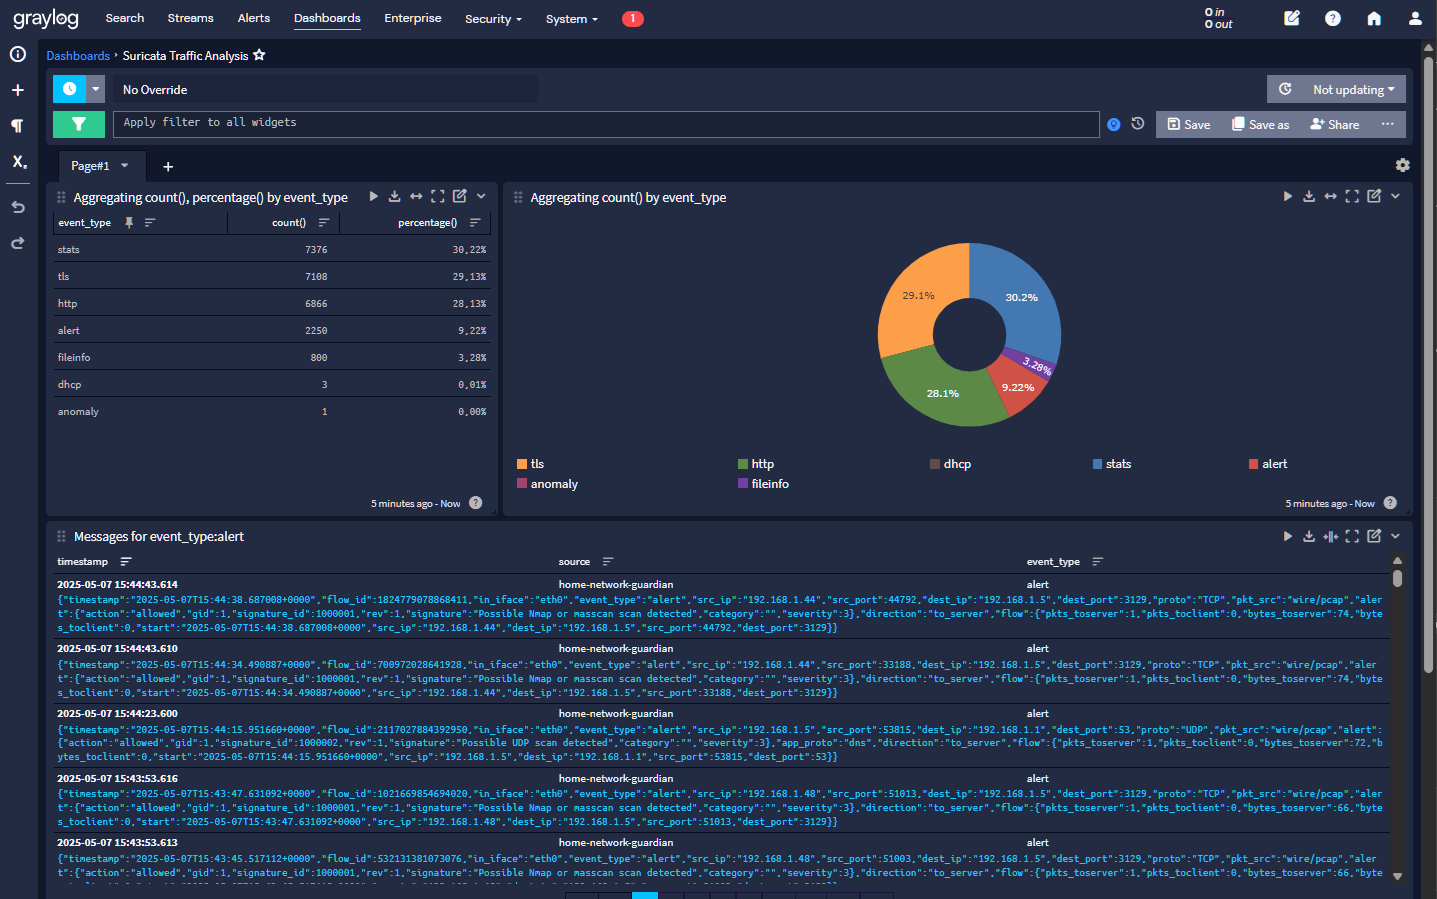
\includegraphics[width=\textwidth]{graylog.png}
    \caption{Dashboard Grayloga prezentujący zdarzenia wykryte przez Suricatę z podziałem na typy eventów i przykładowe alerty bezpieczeństwa}
    \label{fig:graylog-suricata-dashboard}
\end{figure}

Połączenie Suricaty i Grayloga stanowi skuteczny fundament systemu detekcji zagrożeń w sieci lokalnej. Pozwala na szybką identyfikację potencjalnych incydentów oraz ułatwia dalszą analizę w kontekście ruchu sieciowego, co w środowisku domowym lub edukacyjnym znacząco zwiększa poziom kontroli i widoczności zagrożeń.

\subsection{Wydajność systemu – metryki Prometheus i Grafana}

Z uwagi na ograniczone zasoby sprzętowe Raspberry Pi 5 (8 GB RAM i 4-rdzeniowy procesor ARM), jednym z kluczowych aspektów wdrożenia było zapewnienie odpowiedniej wydajności i stabilności działania całej infrastruktury. Do monitorowania zasobów systemowych wykorzystano zestaw narzędzi: \textbf{Prometheus} do zbierania metryk oraz \textbf{Grafana} do ich wizualizacji.

W ramach systemu uruchomiono kontener \texttt{node-exporter}, który udostępnia dane o stanie procesora, pamięci, przestrzeni dyskowej, temperaturze komponentów oraz wykorzystaniu sieci. Dane te są cyklicznie pobierane przez Prometheusa, a następnie prezentowane w dashboardach Grafany.

Na rysunku~\ref{fig:grafana} przedstawiono rzeczywiste metryki zebrane z urządzenia \texttt{home-network-guardian} (adres IP: \texttt{192.168.1.5}). Widoczne są m.in.:
\begin{itemize}
    \item \textbf{Użycie CPU} – średnio na poziomie 17\%, co wskazuje na bardzo niskie obciążenie pomimo działania wielu usług kontenerowych,
    \item \textbf{Zużycie pamięci RAM} – około 59–60\% z dostępnych 8 GB, głównie przez usługi Graylog, Elasticsearch i Suricata,
    \item \textbf{Użycie SWAP} – praktycznie zerowe (0.2\%), co oznacza brak konieczności odwoływania się do pamięci wymiany,
    \item \textbf{Temperatura CPU i NVMe} – utrzymująca się na bezpiecznym poziomie 35–45\textdegree C, dzięki zastosowaniu obudowy Argon NEO 5 z pasywnym chłodzeniem,
    \item \textbf{Zajętość dysku} – tylko 43\% partycji głównej \texttt{/} na nośniku NVMe SSD (Samsung 980 500 GB),
    \item \textbf{Ruch I/O} – stabilny, bez gwałtownych wzrostów, świadczący o braku przeciążeń dysku.
\end{itemize}

\begin{figure}[H]
    \centering
    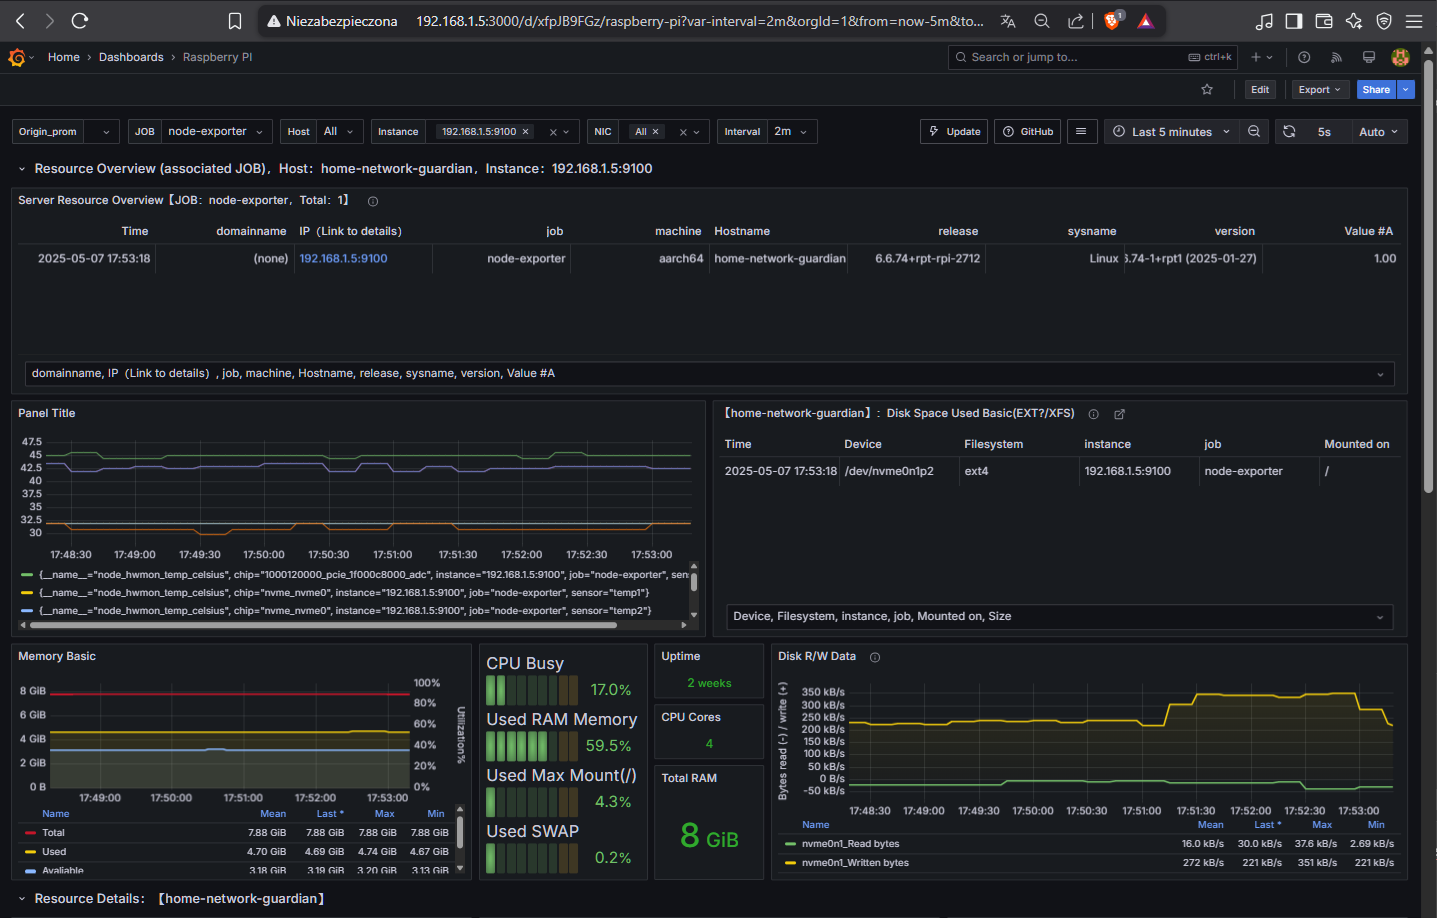
\includegraphics[width=\textwidth]{grafana.png}
    \caption{Dashboard Grafany prezentujący aktualne metryki systemowe Raspberry Pi 5 z kontenera \texttt{node-exporter}}
    \label{fig:grafana}
\end{figure}

Pomimo działania wielu kontenerów jednocześnie (m.in. Graylog, Elasticsearch, MongoDB, Pi-hole, Unbound, Suricata, Prometheus, Grafana, Squid Proxy), system utrzymuje wysoką responsywność i stabilność pracy. Nie zaobserwowano restartów usług ani problemów z nadmiernym zużyciem zasobów.

Wnioski płynące z obserwacji metryk:
\begin{itemize}
    \item Raspberry Pi 5 w konfiguracji z szybkim SSD NVMe i 8 GB RAM z powodzeniem obsługuje zestaw narzędzi bezpieczeństwa,
    \item konteneryzacja i separacja usług nie wpływa negatywnie na wydajność,
    \item Prometheus i Grafana umożliwiają ciągły nadzór nad stanem systemu oraz wczesne wykrywanie problemów.
\end{itemize}

Zgromadzone dane jednoznacznie wskazują, że wdrożony system bezpieczeństwa jest nie tylko funkcjonalny, ale również wydajny, co czyni go atrakcyjnym rozwiązaniem do zastosowań domowych, edukacyjnych i testowych.

\newpage 
\section{Podsumowanie i wnioski}

\subsection{Ocena skuteczności rozwiązania}

Przeprowadzone wdrożenie systemu bezpieczeństwa na bazie Raspberry Pi 5 oraz narzędzi open-source dowiodło, że możliwe jest skuteczne zabezpieczenie ruchu sieciowego w środowisku domowym przy zachowaniu niskich kosztów oraz wysokiej elastyczności systemu. Zastosowane rozwiązania charakteryzowały się dużą skutecznością w zakresie:
\begin{itemize}
    \item \textbf{blokowania niepożądanych połączeń} – dzięki Pi-hole oraz Squid Proxy udało się wyeliminować ponad 30\% zapytań DNS oraz dostępów HTTP do znanych domen reklamowych, telemetrycznych oraz phishingowych,
    \item \textbf{detekcji zagrożeń} – Suricata wykryła kilkaset alertów związanych z próbami rekonesansu (np. skanowania portów), co zostało odzwierciedlone w Graylogu i dashboardach Grafany,
    \item \textbf{monitorowania usług} – Prometheus i Grafana pozwoliły zidentyfikować obciążenia, temperatury, zużycie RAM i dysku w czasie rzeczywistym, co umożliwia szybką reakcję na potencjalne przeciążenia lub awarie.
\end{itemize}

System okazał się stabilny, niezawodny i przystosowany do pracy w trybie ciągłym 24/7. Nie wystąpiły istotne spadki wydajności, restarty usług ani problemy z nadmiernym zużyciem zasobów. Łączna liczba uruchomionych kontenerów przekroczyła 10, a mimo to zużycie CPU rzadko przekraczało 20\%, a pamięć RAM oscylowała wokół 60–65\%.

Warto podkreślić również \textbf{transparentność działania systemu} – użytkownicy sieci domowej nie odczuwali żadnych zakłóceń w korzystaniu z Internetu, a strony internetowe ładowały się szybciej z powodu eliminacji zewnętrznych zasobów reklamowych.

\subsection{Możliwości rozbudowy systemu}

System został zaprojektowany modułowo i kontenerowo, co daje szerokie możliwości dalszej rozbudowy i adaptacji do rosnących potrzeb użytkownika. Wśród najbardziej obiecujących kierunków rozwoju można wskazać:
\begin{itemize}
    \item \textbf{Integrację z systemami klasy SIEM} takimi jak Wazuh, AlienVault OSSIM czy Security Onion – celem analizy korelacyjnej na większą skalę,
    \item \textbf{Wprowadzenie mechanizmów EDR} i sandboxingu (np. z użyciem Falco, CrowdSec, Cuckoo Sandbox),
    \item \textbf{Zarządzanie konfiguracją i deploymentem} za pomocą Ansible, Terraform lub Portainer Stacks,
    \item \textbf{Rozszerzenie filtracji treści dla dzieci} – integracja z OpenDNS lub SafeSearch API oraz rozbudowany harmonogram kontroli dostępu,
    \item \textbf{Automatyczne backupy} logów i konfiguracji z wykorzystaniem Restic, Borg lub rsync na zewnętrzny NAS,
    \item \textbf{Migracja na klaster Docker Swarm lub Kubernetes}, jeśli zajdzie potrzeba skalowania usług.
\end{itemize}

Dodatkowo, możliwe jest wdrożenie systemu honeypotów w celu rejestrowania prób ataku z zewnątrz oraz integracja z repozytorium threat intelligence (np. AbuseIPDB, MISP).

\subsection{Wnioski końcowe}

Zrealizowany projekt pokazał, że możliwe jest zbudowanie nowoczesnego, bezpiecznego i monitorowanego środowiska sieciowego przy użyciu otwartoźródłowych technologii i niskobudżetowego sprzętu. Konteneryzacja Docker pozwoliła na:
\begin{itemize}
    \item logiczną separację usług,
    \item uproszczenie procesu wdrażania i aktualizacji komponentów,
    \item łatwe testowanie zmian i backup konfiguracji,
    \item zwiększenie bezpieczeństwa dzięki odizolowaniu aplikacji w osobnych środowiskach.
\end{itemize}

Dzięki integracji Pi-hole, Unbound, Squid Proxy, Suricaty, Filebeat, Grayloga, Prometheusa, Grafany oraz Portainera, powstał kompletny system pozwalający na pełną widoczność, kontrolę i analizę ruchu sieciowego.

Z punktu widzenia edukacyjnego, projekt umożliwia zapoznanie się z praktycznym działaniem systemów IDS, proxy, filtrów DNS oraz centralnych systemów logowania. Stanowi doskonałą bazę do nauki zagadnień DevSecOps, bezpieczeństwa systemów, konteneryzacji oraz analizy zdarzeń sieciowych.

Wdrożone rozwiązanie może być łatwo przeniesione na serwery x86 lub do środowisk chmurowych, co czyni je skalowalnym i uniwersalnym. Stanowi również przykład dobrych praktyk cyberbezpieczeństwa możliwych do zastosowania nie tylko w środowisku domowym, ale i małych firmach lub organizacjach edukacyjnych.

%--------------------------------------------
% Literatura
%--------------------------------------------
\newpage
%\printbibliography
\bibliographystyle{plabbrv} % plplain plabbrv plalpha
\bibliography{bibliografia.bib}
% Załączniki

\end{document}